
% !TEX root = ../presentation.tex



% ||||||||||||||||||||||
% |||||| The code ||||||
% ||||||||||||||||||||||


\subsection{The code}

\begin{frame}{The code}
    \texttt{AsGRD}, based on \texttt{gevolution}, computes the full metric perturbations with the asymmetron blahblah

    \pause
    \medskip
    Periodic BCs $\Rightarrow$ at least 2 walls. In two dim.: 

\end{frame}



\begin{frame}{Experiments}
    Cubic simulation box of side lengths $L_\#$ (fundamental frequency $k_\#=2\ppi/L_\#$) with $N_\#^3$ lattice points, with initial\textbf{(explain)} perturbation $\epsilon(\tau_\ast, x, y)=\epsast \sin{py}$. Fiducial symmetron parameters are $a_\ast = 0.33$, $\xi_\ast = 3.33\times 10^{-4}$ and $\beta_\ast=1$. Simulation onset is at scale factor $a\ped{i} \gtrsim  a_\ast$, and we finish at $a\ped{f}=0.50$.
    

    \uncover<2-3>{
    \begin{table}
        {\small{\begin{tabular}{@{}cl@{}}
            % \pause
            \uncover<2-3>{
            \simI & $\epsast= 0.08L_\#$, $p=2k_\#$, $L_\# \approx 1~\Mpch[G]$, $N_\# = 768 $, $a\ped{i} \simeq a_\ast + 0.003$ \\
            \midrule}%
            % \pause 
            \uncover<3>{%
            \simII & $\epsast\to 0.12L_\#$ \\
            \simIII & $N_\# \to 900$\\
            \simIV & $L_\# \to 1.4~\Mpch[G] $ \\
            \simV & $p\to 3k_\#$, $\epsast\to 0.06L_\#$, $N_\# \to 900$\\
            % \simVI & \\
            \simVII & $(a\ped{i}-a_\ast)\to 0.001 $}
        \end{tabular}}}
    \end{table}}

    % \only<4>{
    % \begin{figure}
    %     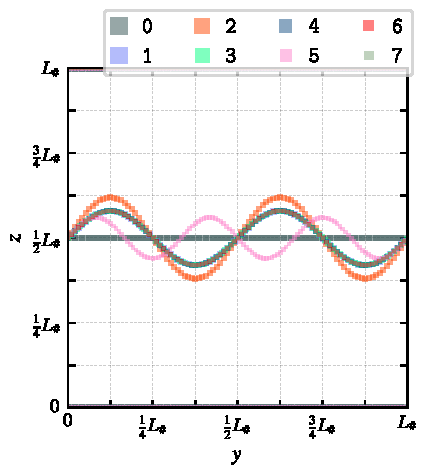
\includegraphics[width=0.4\textwidth]{../../figs/Methodology/initial_perturbations.pdf}
    % \end{figure}
    % }

\end{frame}


\begin{uioimageframe}{../../figs/Methodology/initial_perturbations.pdf}
    {
    \newcommand{\INC}[1]{\(#1\mathcolor{uiogreen2}{\nearrow}\)}
    \newcommand{\DEC}[1]{\(#1\mathcolor{uiopink2}{\searrow}\)}
    \begin{table}
        {\small{\begin{tabular}{@{}cl@{}}
            % \pause
            \uncover<2>{\simO & \DEC{\epsast }} \\
            \simI & ---\\
            % \midrule
            \simII & \INC{\epsast}\\
            \simIII & \INC{N_\#}\\
            \simIV & \INC{L_\#} \\
            \simV & \INC{p} \,\,\, \DEC{\epsast} \,\,\, \INC{N_\#} \\
            \uncover<2>{\simVI & \DEC{\xi_\ast} \\}
            \simVII &  \DEC{(a\ped{i}-a_\ast)}
        \end{tabular}}}
    \end{table}}
\end{uioimageframe}


% ||||||||||||||||||||||
% |||||| Findings ||||||
% ||||||||||||||||||||||

\subsection{Findings}

\begin{frame}{Time measures}
    % Time variables
    \begin{description}
        \item[\descItem{scale factor} ] $\only<3>{\mathcolor{uioblue1}}{a}= \pclosed{1+\redshift}^{-1} = a_\ast s^\alpha$
        \item[\descItem{cosmic redshift} ] $\redshift=1/a - 1$
        \item[\descItem{conformal time} ] $s= \tau/\tau_\ast$
        \item[\descItem{scale-dependent time parameter} ] $\only<3>{\mathcolor{uioblue1}}{t_\omega} \equiv \omega (s-1) = p(\tau-\tau_\ast)$
        \item[\descItem{phase-transition time-scale} ] $\chi_+ \equiv \sqrt{1-\upsilon} = \sqrt{1-{(a_\ast/a)}^3}= \sqrt{1-s^{-3\alpha}}$ 
    \end{description}
    \uncover<2->{
    \bigskip
    Matter domination $\leftrightarrow$ $\alpha=2$}
\end{frame}



% \begin{frame}{idk}
\uiobigimage{Analytical vs. simulated wall position}{../../figs/Findings/eps_diff_sims_combi.pdf}{$e\equiv\varepsilon/\epsast$, $\Delta e \equiv \abs*{\epsA-\epsB}$} 
% \uiofullpageimage{../../figs/Findings/eps_diff_sims_combi.pdf}
% \end{frame}



\begin{frame}{Main results}
    % We use $e\equiv\varepsilon/\epsast$

    % \begin{minipage}{\textwidth}
    % \begin{table}
    % \begin{threeparttable}
    %     {
    %     \newcommand\YAY{\textcolor{G1}{yes}}
    %     \newcommand\NAY{\textcolor{R1}{no}}
    %     \newcommand\MAY{\textcolor{O1}{yes\tnote{*}}}
    %     % \renewcommand{\thefootnote}{\fnsymbol{footnote}}
    %     % -----------------------
    %     \begin{tabular}{@{}lcc@{}}
    %         & \tabHeading{Calculation} & \tabHeading{Simulation} \\
    %         \toprule
    %         % -----------
    %         \uncover<1->{$e$ independent of $\epsast$ & \YAY & \NAY } \\
    %         \uncover<2->{$e\not\sim s^{-5/2}\Cylindrical[-5/2](\omega s)$ & \YAY & \YAY} \\
    %         \uncover<3->{($e$ vs.~$t_\omega$)-plot indep. of parameters &\YAY & \MAY} \\
    %         % & \dots & \dots  \\
    %         \bottomrule
    %     \end{tabular}
    %     \uncover<3->{\begin{tablenotes}
    %         \item[*] To some extent.
    %     \end{tablenotes}}
    %     }
    % \end{threeparttable}
    % \end{table} 
    % \end{minipage}

    \begin{table}
    \begin{threeparttable}
        {
        \newcommand\YAY{\textcolor{G1}{yes}}
        \newcommand\NAY{\textcolor{R1}{no}}
        \newcommand\MAY{\textcolor{O1}{yes\tnote{*}}}
        % \renewcommand{\thefootnote}{\fnsymbol{footnote}}
        % -----------------------
        {\small{\begin{tabular}{@{}lcc@{}}
            & \tabHeading{Calculation} & \tabHeading{Simulation} \\
            \toprule
            % -----------   
            \tabSubheading{Wall position,} $e= \varepsilon/\epsast$ & $\epsA[e]$ & $\epsB[e]$\\
            \midrule
            % -----------
            \uncover<1->{$e$ independent of $\epsast$ & \YAY & \NAY } \\
            \uncover<2->{$e\not\sim s^{-5/2}\Cylindrical[-5/2](\omega s)$ & \YAY & \YAY} \\
            \uncover<3->{($e$ vs.~$t_\omega$)-plot indep. of parameters &\YAY & \MAY} \\
            % & \dots & \dots  \\
            \midrule
            \tabSubheading{Gravitational waves} & $\hpA$ $(\hpB)$ & $\hpC$ \\
            \midrule
            \uncover<3->{? &\YAY & \MAY} \\
            \bottomrule
        \end{tabular}}}
        \uncover<3->{\footnotesize{\begin{tablenotes}
            \item[*] To some extent.
        \end{tablenotes}}}
        }
    \end{threeparttable}
    \end{table} 

\end{frame}


\begin{frame}
    $\epsA$ vs $\ALIASepsA$ vs $\varepsilon\ap{NG}$
\end{frame}

